\documentclass{crebss}
\usepackage{array}
\usepackage{longtable}
\usepackage{microtype}
\newcolumntype{L}[1]{>{\raggedright\arraybackslash}p{#1}}
\newcommand{\rankic}{\mathrm{RankIC}}
\newcommand{\qlike}{\mathrm{QLIKE}}
\setcounter{page}{1}
\setcounter{secnumdepth}{3}
\renewcommand\thisnumber{x}
\renewcommand\thisyear{202x}
\renewcommand\thisvolume{x}
\renewcommand\datereceived{under review}
\renewcommand\dateaccepted{under review}
\renewcommand\dateavailable{under review}
\renewcommand\doinumber{assigned after acceptance}
\renewcommand\type{Original scientific paper}
\renewcommand\JEL{C52, C53, G17}

\begin{document}
\raggedbottom
\markboth{Anonymous}{Mechanism activation and forecast value}
\title{From Mechanism Activation to Forecast Value: A Multi-Study Audit on Public Equity Panels}
\author[]{}
\address{}
\keywords{ablation, financial forecasting, forecast comparison, model selection, negative results}

\begin{abstract}
Architectural novelty in financial forecasting is hard to evaluate when weaker variants disappear from view and gains may reflect extra computation or comparator choice. We turn five completed studies into a common mechanism-value audit covering expert communication, disagreement arbitration, analog retrieval, stress-conditioned correction, and delayed hierarchical pooling on three public daily equity panels. The archive contains 111 fitted model cells and fifteen study--panel evaluations. Because the studies target cross-sectional return ranking, conditional return quantiles, and a five-day daily-return variance proxy, we retain each proper score rather than pool incommensurate effects. Every full mechanism is evaluated against a same-information reduction and strong external controls; uncertainty is estimated over chronological date blocks; and four-cell designs identify component interactions. No full mechanism cleared its study-specific broad success gate, and none of the fifteen factorial interactions had a favorable panel-level interval. The mechanisms expose four bottlenecks: insufficient separation among actions, weak alignment with future loss, improvement within an inadequate forecast family, and adaptation that contracts toward static pooling after delayed feedback. The resulting map converts adverse experiments into reusable design evidence.
\end{abstract}

\maketitle

\section{Introduction}

The development of a financial forecasting model often leaves behind a long series of plausible mechanisms. A researcher may add specialist communication, disagreement-sensitive routing, retrieval from similar episodes, multiple adaptation speeds, or cross-asset pooling. Each addition has a coherent story. Each can also generate visually persuasive internal diagnostics. Yet the scientific question is narrower: does the mechanism improve the prespecified forecasting objective beyond controls that receive the same information?

This distinction matters in finance because the space of models, targets, panels, and evaluation choices is large. Repeated search can turn ordinary sampling variation into an apparently successful specification, a concern that motivates reality checks, multiple-testing corrections, and replication work in empirical finance \citep{white2000reality,harvey2016cross,hou2020replicating}. The publication process supplies an additional filter. Negative results have become less visible in many disciplines \citep{fanelli2012negative}, even though they can identify when an appealing mechanism fails to add information.

We report the complete evidence from five sequential forecasting studies. The studies were not designed as independent replications, and they should not be read as five draws from a common population. They share three public daily equity panels and were developed over time. They also address different targets. The value of the synthesis is therefore diagnostic rather than meta-analytic: each study contains a fixed full model, matched controls, a four-cell mechanism design, dated out-of-sample predictions, and an evidence archive that preserves adverse results. This common structure lets us examine how different ideas failed.

The audit population is every completed study in the project archive between 29 September and 2 October 2026 that used all three panels, retained a four-cell mechanism design, and returned a complete evidence archive. Five studies met these criteria and none was omitted. Results from earlier studies were known when later mechanisms were designed; all fifteen cells are therefore treated as related development evidence.

Across the five studies, no full mechanism met its study-specific broad success condition. Local signals existed, but they were comparator-specific, panel-specific, or reproduced by simpler cells. The common diagnostic pattern was a gap between an active module and an identified contribution. A router could change its output without choosing meaningfully different experts. Communication could be present in the graph while its numerical contribution remained negligible. A correction branch could improve a weak anchor yet remain inferior to an equally informed statistical or neural control. A dynamic pool could move away from static weights while still failing to beat the best frozen forecast.

This article contributes a mechanism-value framework that separates four questions: whether a module runs, creates differentiated actions, improves a matched comparator, and yields the proposed interaction. Across all 111 fitted cells, it produces a five-regime taxonomy---dormancy, non-translation, redundant activity, family weakness, and adaptive contraction---that links results to redesign decisions. It also yields governance rules based on same-information reductions, date-level inference, matured feedback, and separation of within-family gains from broad forecast value.

\section{Literature review and analytical framework}

Forecast evaluation is a decision problem. A model should be judged by a loss function chosen for the target and use case, rather than by the visual complexity of its architecture \citep{gneiting2011point}. For variance forecasts, proxy choice and loss choice are especially consequential. QLIKE belongs to the class of losses designed to preserve useful comparisons under conditionally unbiased but noisy volatility proxies \citep{patton2011volatility}. For conditional quantiles, pinball loss is consistent with the target quantile. For cross-sectional ranking, a date-level rank correlation measures whether the ordering of assets is correct. These objectives are not interchangeable.

The same caution applies to uncertainty. Adjacent financial targets overlap in time and assets within a date share market shocks. Treating all asset--date observations as independent would overstate precision. Each study therefore uses dates as the inferential unit and chronological blocks for uncertainty. This follows the broader principle behind forecast-comparison procedures: comparisons should be made on matched observations with dependence accounted for \citep{diebold1995predictive,hansen2011mcs}.

Mechanism attribution creates a second problem. A full model that beats a simple baseline does not establish that two proposed modules complement each other. A four-cell design can distinguish a base model, each module alone, and both together. Let the raw interaction be
\[
  J = M_{11}-M_{10}-M_{01}+M_{00}.
\]
We report $I=J$ for higher-is-better scores and $I=-J$ for losses, so a positive $I$ always favors complementarity. Even then, a favorable interaction does not imply that the full model is better than an external baseline. The interaction and the total effect answer different questions.

Finally, online or adaptive mechanisms face an information clock. Feedback from an origin cannot be used until its complete target horizon has elapsed. Delayed-feedback learning is a distinct statistical setting \citep{joulani2013delayed}. Each adaptive study in this audit updates only from matured outcomes. This prevents a common form of look-ahead but does not guarantee that the adaptive rule will help.

\subsection{Activation, alignment, and forecast risk}

The distinction between an active module and a useful module can be written directly in forecast-risk terms. Let $b_t$ denote the matched baseline forecast at date $t$, let $d_t$ be the change produced by a proposed mechanism, and let $f_t=b_t+d_t$ be the full forecast. For a target $y_t$ and the study's proper loss $\ell$, the population improvement of the full mechanism over its matched reduction is
\[
  \Delta = \operatorname{E}\!\left[\ell(y_t,b_t)-\ell(y_t,b_t+d_t)\right].
\]
An activation diagnostic instead measures a quantity such as $A=\operatorname{E}|d_t|$, route entropy, message energy, or the dispersion of internal weights. Except for the degenerate case $A=0$, activation places no sign restriction on $\Delta$. It establishes that the mechanism moves the forecast, not that the movement is directed toward lower risk.

For a smooth convex loss, a local expansion around the matched forecast makes the missing requirement explicit:
\[
  \Delta \approx -\operatorname{E}[g_t d_t]
  -\tfrac{1}{2}\operatorname{E}[h_t d_t^2],
  \qquad
  g_t=\partial_b\ell(y_t,b_t),\quad h_t=\partial_b^2\ell(y_t,b_t)\geq 0.
\]
The first term rewards alignment between the mechanism's correction and the negative loss gradient. The second term penalizes movement through the curvature of the loss. A module can therefore be active and economically interpretable while producing no gain if its corrections are weakly aligned, excessively variable, or concentrated in dates where the matched model is already adequate. Pinball loss is not differentiable at zero residual, but the same argument holds with a subgradient. Rank-based scores do not admit the same local expansion, yet the analogous requirement remains: altered pairwise orderings must be correct often enough to offset newly introduced inversions.

The four-cell interaction asks a further question. Suppose modules $A$ and $B$ each create a forecast change. Their performance interaction is favorable only when using them together creates value beyond the sum of their separate contributions. Two modules may both activate and still have a near-zero interaction because they encode the same state information. A negative interaction can arise when one module changes the region in which the other was calibrated or when their errors reinforce one another. This explains why a factorial result cannot be inferred from two attractive mechanism plots.

Adaptive modules face an additional burden. Their attainable gain must exceed the estimation error of the adaptive rule, the information lost while outcomes mature, and the cost of transferring a validation relation into a later regime. Shrinkage and multiple memory scales can reduce those costs, but they cannot create predictive information absent from the frozen forecast bank. The empirical role of the audit is to determine which side of this trade-off dominates on common dates.

\subsection{Identification under nested information sets}

A mechanism can appear useful for three different reasons. It may introduce genuinely new information, transform an existing information set more effectively, or select among existing forecasts in states where their relative quality changes. These explanations have different empirical requirements. Let $\mathcal{I}_t$ denote everything available at the forecast origin. If a full model and its reduction use different versions of $\mathcal{I}_t$, their performance difference mixes information content with architecture. If they use the same information but receive different fit periods or optimization opportunities, the difference also contains a training-opportunity effect. A matched reduction is therefore most informative when it shares the target, features, forecast origins, eligible assets, fit window, and loss, while removing only the proposed operation.

This nested design gives the incremental comparison a clear interpretation. The contrast asks whether the mechanism extracts value from information already available to both cells. It does not require the reduction to be the strongest model in the literature. In fact, an extremely weak baseline can obscure attribution: almost any competent full model may beat it, even when the proposed module is irrelevant. Conversely, an external model can be an excellent forecast yet a poor attribution control if it uses a different representation or training protocol. The audit therefore assigns distinct roles to the matched reduction and the strong external comparator. The first identifies the contribution of the mechanism within its family; the second asks whether that family is worth using.

The factorial cells refine the same logic. Comparing the full cell only with the base cell attributes their combined difference to two modules and their interaction at once. The two single-module cells reveal whether one component reproduces the apparent gain and whether the second adds anything after the first is present. This distinction matters when a persuasive story joins modules that are individually sensible. Communication and routing may both operate, yet routing may simply recover what a risk-only cell already knows. Two memories may retrieve different episodes, yet a plain dual-memory model may already capture the useful part of that difference. The factorial is thus an identification device, not merely an ablation checklist.

No single comparator answers all three questions. A matched reduction can show incremental value while the entire family remains dominated; an external comparator can show competitiveness without identifying the proposed module; and a favorable interaction can coexist with a full model that is poor in absolute terms. Requiring all three creates a demanding success condition, but it prevents architectural novelty from being mistaken for predictive content. This is especially important after repeated model development, when flexible specifications create many plausible routes to an attractive point estimate.

\subsection{When conditional value disappears in the aggregate}

Many financial mechanisms are motivated by a conditional claim. Communication should help when specialists hold complementary information. Arbitration should help when forecasters disagree. Retrieval should help when a current state has a close historical analog. Stress corrections should help in adverse regimes, and adaptive pooling should help when relative model quality changes. Let $S_t$ mark the state in which a mechanism is expected to help. Its unconditional improvement can be written as the frequency-weighted combination $\Pr(S_t)\Delta_1+[1-\Pr(S_t)]\Delta_0$, where $\Delta_1$ and $\Delta_0$ are improvements inside and outside the target state. A large conditional gain can vanish if the state is rare, if losses outside it are adverse, or if the deployed selector cannot identify it prospectively.

This expression separates the quality of a correction from the quality of its gate. Even if an oracle could identify useful interventions, a learned gate must estimate the state from past-only variables. False positives apply a correction when the base forecast is adequate; false negatives miss the dates that motivated the mechanism. Near the decision boundary, small estimation errors can switch an intervention on or off, adding variance that is absent from an always-on or always-off control. A gate should therefore be compared with rules that match its adoption rate as well as with unrestricted alternatives. Otherwise, an apparent gate effect may reflect the amount of intervention rather than the information used to choose it.

The same reasoning explains why strong activation plots can coexist with weak loss differences. Route entropy, expert disagreement, memory diversity, and correction magnitude describe the supply of possible actions. Forecast value depends on the covariance between those actions and avoidable future error. A model may discover stable market states that are interesting but already reflected in its anchor forecast. It may also detect genuine disagreement that is symmetric around the truth and therefore unhelpful for choosing a winner. Internal separation is evidence that representations differ; it is not evidence that the differences are ordered by future loss.

\subsection{Complexity, delayed feedback, and the hurdle rate for adaptation}

Model complexity is not only a parameter count. For adaptive financial systems it also includes the number of candidate forecasts, routing choices, memory scales, thresholds, state definitions, and comparisons considered during development. Each choice consumes validation information. A model with few trainable weights can still have a large effective selection burden when many readouts and gates are examined. This burden is particularly consequential in daily panels because the number of distinct market dates is much smaller than the number of asset--date rows.

Delayed targets raise the hurdle further. With a five-date horizon, the error of a forecast made today is unavailable until the entire target matures. The deployed rule must act during that interval without learning from its most recent decisions. Overlapping targets also make adjacent errors dependent, so a long table of asset observations does not imply an equally long history of independent feedback. Short memories can react quickly after labels mature but estimate relative quality noisily. Long memories reduce variance but may average across regimes. Multiple memories offer a compromise only if the routing signal can identify which scale is currently relevant.

These costs imply a practical hurdle rate. A new module must generate enough aligned predictive information to pay for estimation variance, delayed learning, calibration error, and regime transfer. Regularization, shrinkage, and conservative gates lower the cost, but they may also contract the deployed model toward a static rule. Such contraction is rational when evidence is weak; it becomes an empirical warning when the paper's contribution depends on strong adaptation. The important quantity is therefore not how far the architecture could move, but how much useful movement survives validation and remains beneficial on untouched dates.

\section{Methods}

\subsection{Panels and evidence units}

All five studies used three public daily equity panels, denoted SP500, KDD17, and ACL18. The SP500 panel contains current index constituents and is not a survivorship-free historical universe. KDD17 and ACL18 are public stock panels associated with earlier forecasting benchmarks. Each study used chronological fit, validation, and test segments, and test-time asset eligibility depended on information available by the forecast origin. Because the same panels recur across studies, the fifteen study--panel cells are related development evidence rather than independent replications.

The raw SP500, KDD17, and ACL18 files span 2010--2024 (502 symbols), 2007--2016 (50 symbols), and 2012--2017 (88 symbols), respectively. Per-date eligibility is smaller because an asset must have sufficient past observations. The public acquisition records are the SP500 CC0 release \citep{mvd_sp500}, the KDD17 release accompanying Adv-ALSTM \citep{feng2019enhancing}, and the ACL18 StockNet release \citep{xu2018stock}. File hashes, source URLs, and the exact chronological split tables are reported in the supplement.

The returned archives include source hashes, data hashes, configuration files, dated predictions or scores, model histories, paired inference, factorial outputs, figures, and failure records. Every recorded fit completed. Table~\ref{tab:inventory} summarizes the workload. The total of 111 refers to fitted backbones or neural cells; statistical estimation and inexpensive frozen readouts are additional.

\begin{table}[htbp]
\centering
\caption{Completed study inventory.}
\label{tab:inventory}
\small
\begin{tabular}{p{1.6cm}p{3.2cm}p{2.6cm}rrp{3.1cm}}
\toprule
Study & Forecast target & Primary score & Fits & Hours & Full mechanism \\
\midrule
C3R & Cross-sectional future-return ranking & Date-level $\rankic$ & 33 & 0.594 & Residual expert exchange and coalition-risk routing \\
DARC & Cross-sectional future-return ranking & Date-level $\rankic$ & 18 & 0.108 & Pairwise disagreement arbitration and advantage gating \\
CARE & Three conditional return quantiles & Mean pinball loss & 24 & 0.903 & Dual analog memory and tail-sensitive routing \\
MOSAIC & Five-day daily-return variance proxy & Mean QLIKE & 21 & 0.332 & Downside and market-stress correction branches \\
DASH-V & Five-day daily-return variance proxy & Mean QLIKE & 15 & 0.409 & Delayed hierarchical pooling with multiple memories \\
\bottomrule
\end{tabular}
\end{table}

\begin{table}[htbp]
\centering
\caption{Study-specific evaluation design. All reported test intervals use 5,000 chronological moving-block draws with block length 20.}
\label{tab:design}
\scriptsize
\setlength{\tabcolsep}{2pt}
\begin{tabular}{p{1.3cm}p{4.2cm}p{4.2cm}p{4.2cm}}
\toprule
Study & Target and horizon & Comparator family & Comparison multiplicity \\
\midrule
C3R & Five-day adjusted-open return ordering; date-level RankIC & Six adapted neural controls and four C3R reductions & Ten full-model comparisons per panel adjusted by Holm; factorial interaction reported separately \\
DARC & The same five-day return-ordering target; date-level RankIC & Six adapted neural controls and seven frozen readouts & Thirteen full-model comparisons per panel and split adjusted by Holm; factorial reported separately \\
CARE & 10th, 50th, and 90th percentiles of five-day adjusted-open return; mean pinball loss & Historical and market analogs, four neural quantile controls, and three CARE reductions & Nine comparisons per panel and split; 27 cross-panel comparisons per split adjusted by Holm \\
MOSAIC & Mean of the next five squared daily adjusted-close log returns times 10,000; QLIKE & Six statistical controls, three neural or mixture controls, and three MOSAIC reductions & Twelve comparisons per panel and split; 36 cross-panel comparisons per split adjusted by Holm \\
DASH-V & The same five-day daily-return variance proxy; QLIKE & Five statistical, five neural, four pooling controls, and three DASH-V reductions & Seventeen panel comparisons plus the recorded five-comparison family and fifteen cross-panel hypotheses \\
\bottomrule
\end{tabular}
\end{table}

\subsection{Five mechanism tests}

\textbf{C3R.} Four role-specialized experts produced asset scores. The full cell allowed recipient-conditioned residual messages with a no-message option, then learned the relative risk of candidate communication coalitions from a held-out chronological interval. Its matched cells separated communication and coalition-risk supervision. Literature-inspired common-protocol adaptations of StockMixer, MASTER, MIGA, MERA, and MAFS supplied external controls \citep{fan2024stockmixer,li2024master,yu2024miga,liu2025mera,huang2025mafs}; none is presented as an original-author protocol reproduction. The main outcome was date-level RankIC.

\textbf{DARC.} Six frozen forecasters supplied candidate rankings. The proposed readout focused computation on expert disagreements, converted pairwise preferences into a completed ranking, and used matured historical advantage to gate the nonlinear arbitration. Matched readouts included equal rank, static calibration, recent performance, uniform pair voting, and a global weighted-rank reduction. The factorial separated pair-specific arbitration from the advantage gate.

\textbf{CARE.} The model predicted the 10th, 50th, and 90th percentiles of future returns. One memory retrieved earlier market contexts; the other retrieved earlier trajectories of the same stock. Specialist recurrent experts and a shared temporal fallback produced central and interval-width proposals. The factorial separated dual memory from tail-sensitive routing. Historical quantiles, market analogs, and four common-protocol neural quantile models served as controls.

\textbf{MOSAIC.} A positive multiscale variance anchor received two constrained corrections: an own-downside branch and a market-stress branch. The full cell included both branches and an explicit interaction. Statistical HAR-type controls, persistence, neural controls, and a common-protocol RG-ResMoE adaptation \citep{ye2026rgresmoe} received the same daily information. HAR models are natural controls because heterogeneous autoregression explicitly represents volatility persistence at several horizons \citep{corsi2009har}.

\textbf{DASH-V.} Ten frozen statistical and neural forecasts were combined by validation-trained static QLIKE weights and by delayed adaptive rules. The full cell pooled global and asset-local relative losses, estimated cross-asset shrinkage on validation, and mixed fast, medium, and slow memories. Four factorial cells isolated hierarchy and multiple memories. This design is related to adaptive mixtures of experts \citep{jacobs1991mixtures} and concept-drift adaptation \citep{gama2014drift}, but its empirical question was narrower: whether partial pooling makes short-memory adaptation of frozen variance forecasts more reliable.

\subsection{Evaluation rules}

We retain each study's original target and loss. For RankIC studies, positive differences favor the proposed model. For pinball loss and QLIKE, lower values are better; reported ``improvements'' are comparator loss minus full-model loss. Moving-block intervals preserve chronological dependence. Multiplicity adjustments are interpreted within the comparison family defined in each archive. We do not average ranks, $p$-values, or effect sizes across tasks.

We classify evidence at four levels. \emph{Execution} asks whether the module completed and produced finite outputs. \emph{Activation} asks whether it changed internal states or forecasts. \emph{Incremental value} asks whether it beat a matched reduction on common dates. \emph{Broad value} asks whether it also beat the strongest recorded comparators across panels. Only the last level supports a general performance claim.

Figure~\ref{fig:model-mechanisms} places the five implemented mechanisms in one compact plate. The diagrams identify where each full model can depart from its matched reduction; the experimental sections then test whether those departures align with lower out-of-sample loss. Execution and activation remain engineering checks, whereas incremental and broad value require common-date comparisons.

\begin{figure}[H]
\centering
\begin{minipage}{0.485\textwidth}\centering
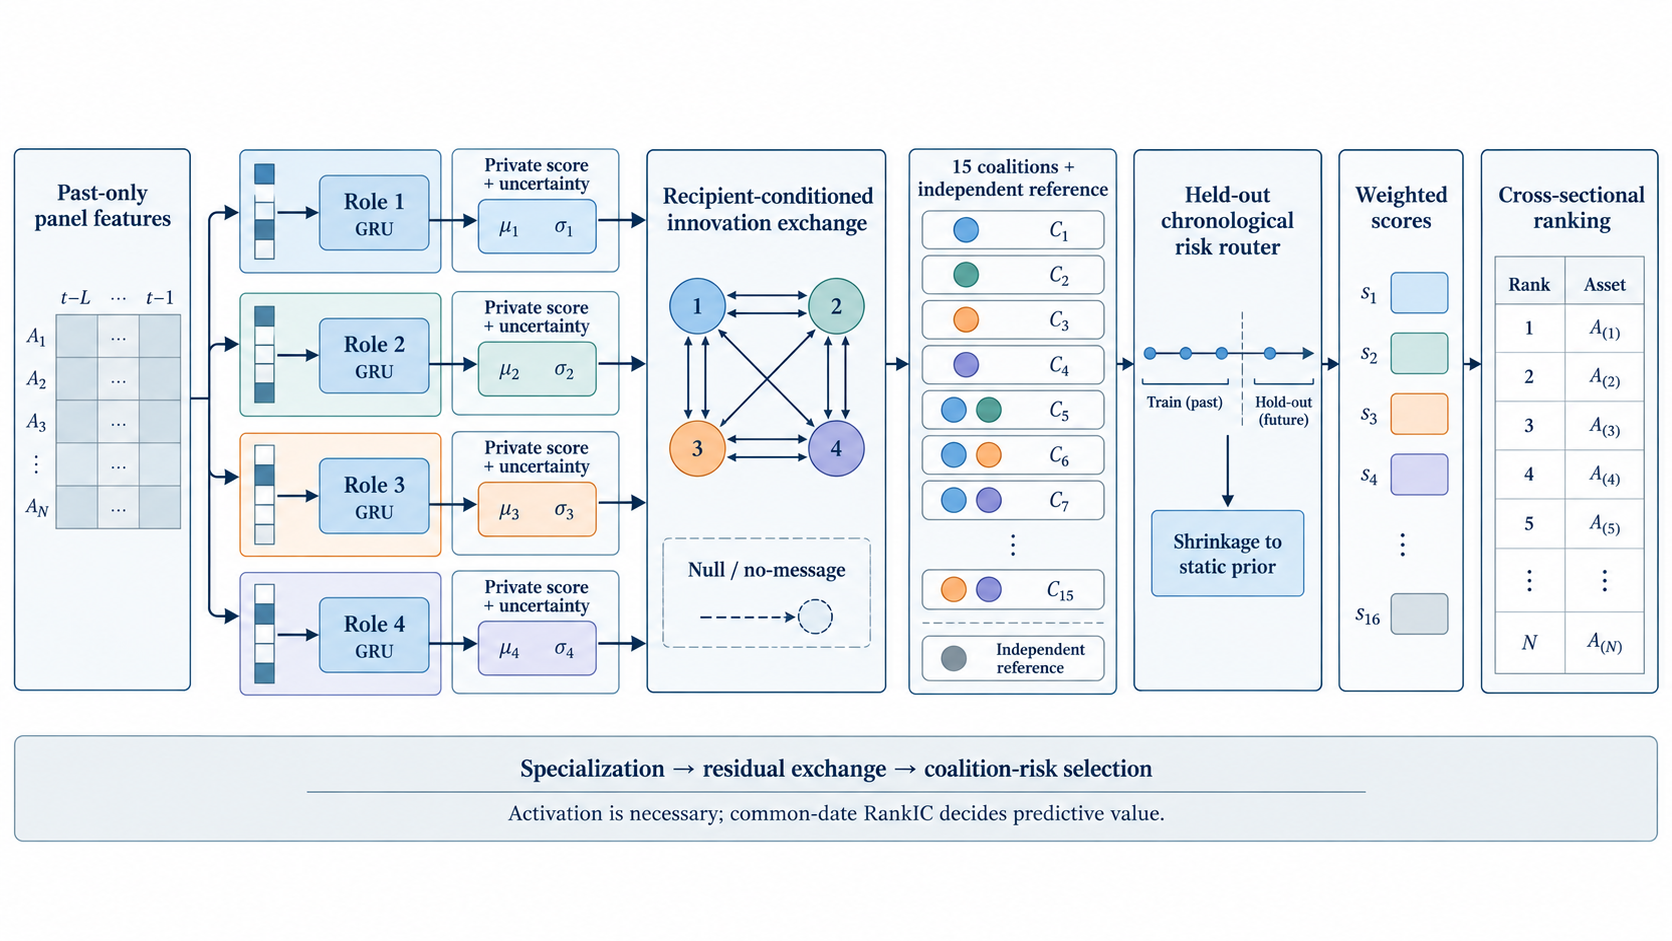
\includegraphics[width=\linewidth]{c3r_mechanism.png}\\[-1mm]\scriptsize (a) C3R
\end{minipage}\hfill
\begin{minipage}{0.485\textwidth}\centering
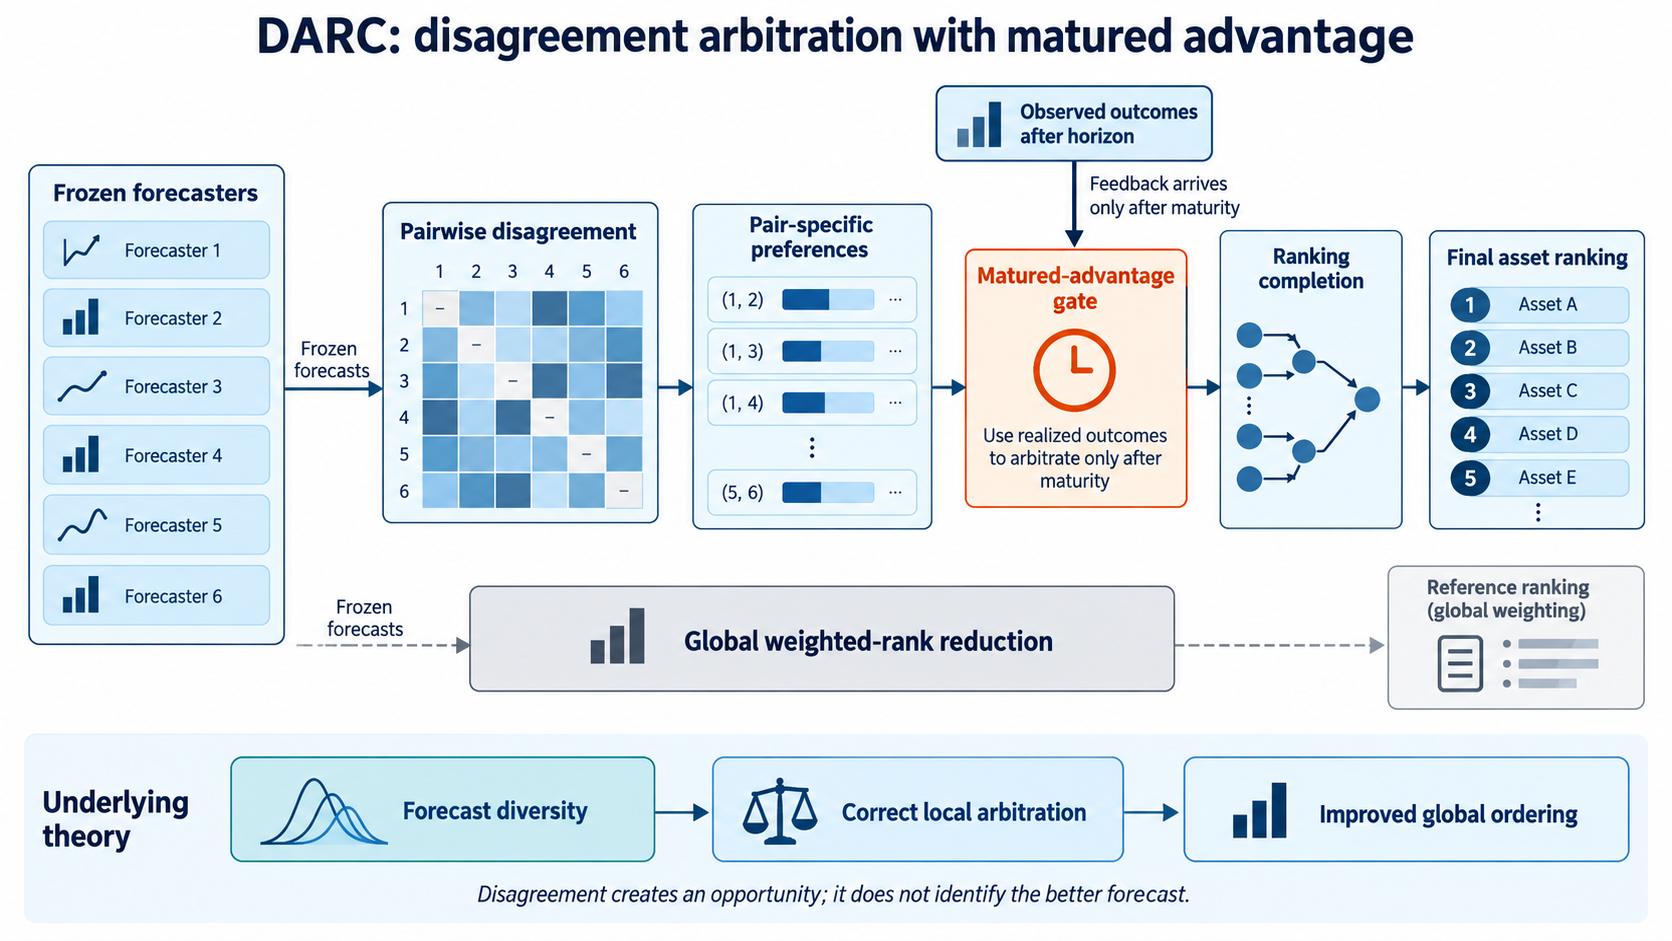
\includegraphics[width=\linewidth]{darc_mechanism.png}\\[-1mm]\scriptsize (b) DARC
\end{minipage}\\[2mm]
\begin{minipage}{0.485\textwidth}\centering
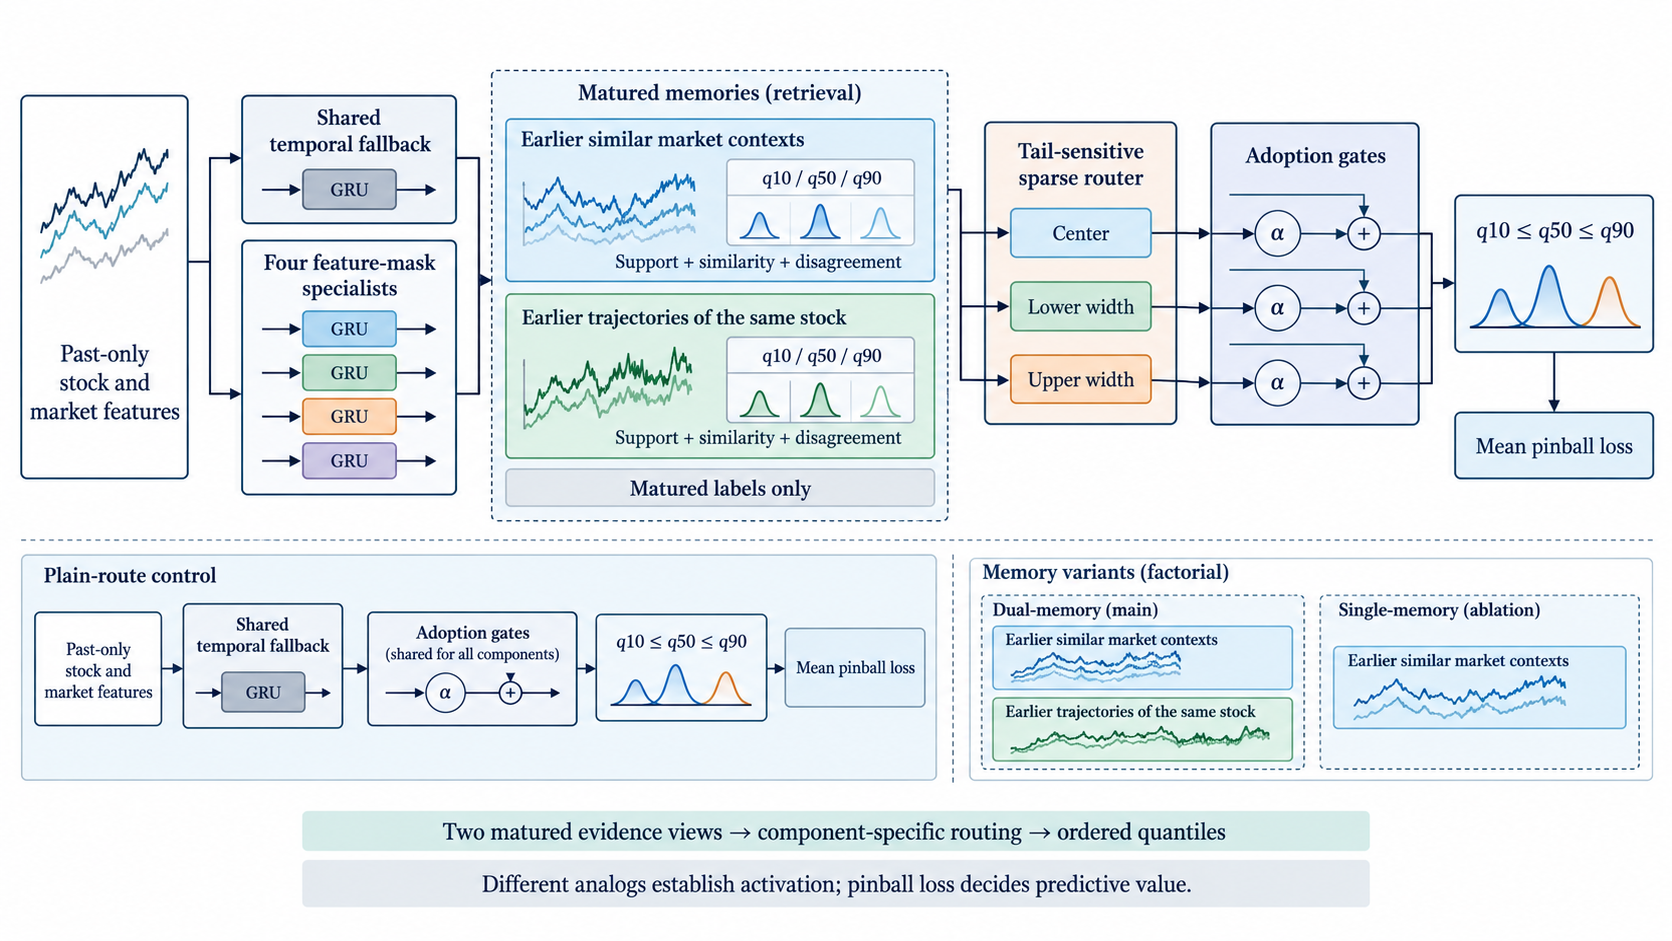
\includegraphics[width=\linewidth]{care_mechanism.png}\\[-1mm]\scriptsize (c) CARE
\end{minipage}\hfill
\begin{minipage}{0.485\textwidth}\centering
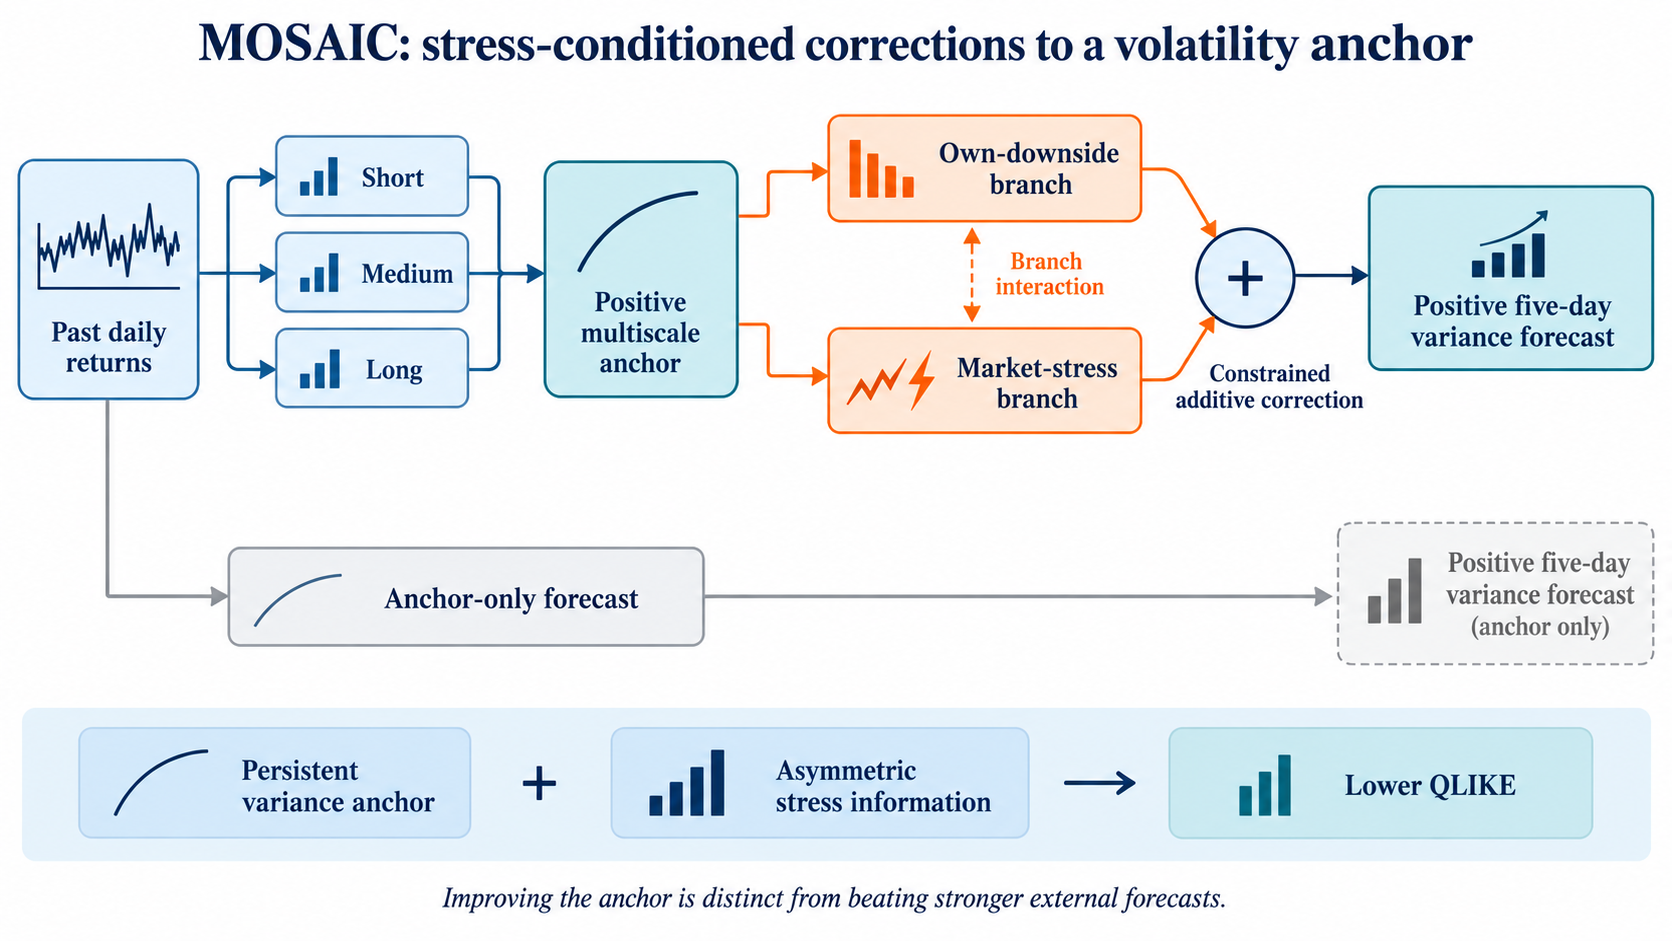
\includegraphics[width=\linewidth]{mosaic_mechanism.png}\\[-1mm]\scriptsize (d) MOSAIC
\end{minipage}\\[2mm]
\begin{minipage}{0.485\textwidth}\centering
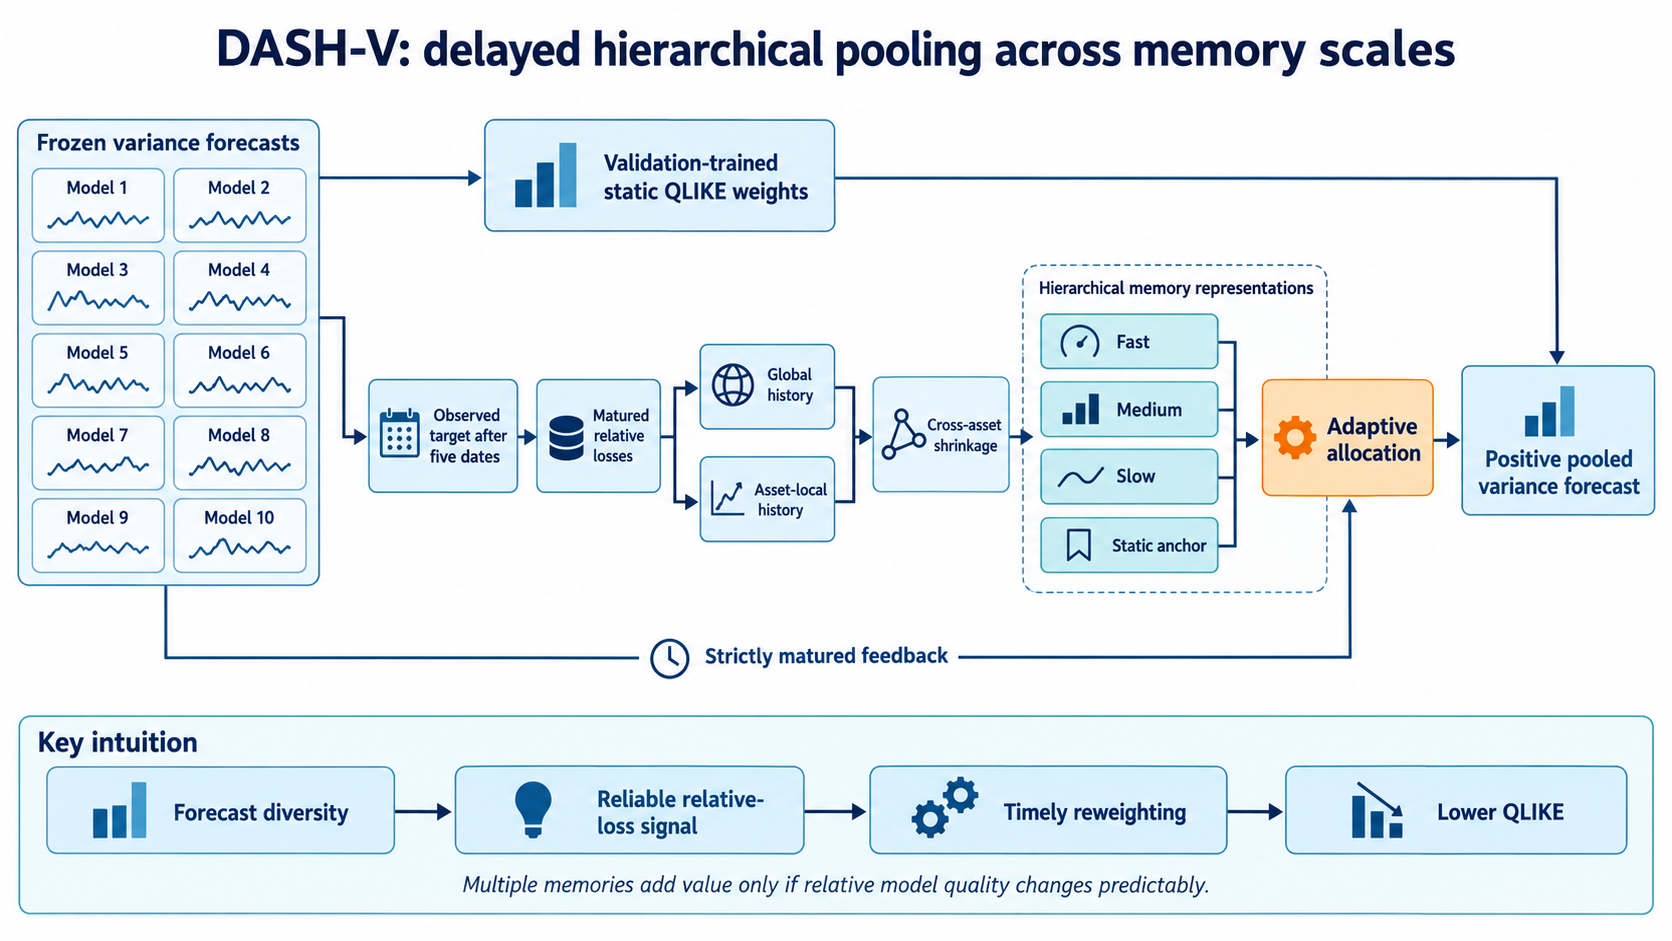
\includegraphics[width=\linewidth]{dashv_mechanism.png}\\[-1mm]\scriptsize (e) DASH-V
\end{minipage}
\caption{Implemented mechanism plate. C3R uses residual expert exchange and coalition-risk routing; DARC converts gated pairwise preferences into a completed ranking; CARE combines two matured analog memories with component-specific quantile routing; MOSAIC applies constrained stress corrections to a positive multiscale anchor; and DASH-V adapts a frozen forecast pool through delayed, partially pooled multi-scale loss memories. The diagrams describe computation; predictive evidence appears in Table~\ref{tab:main} and the factorial figures.}
\label{fig:model-mechanisms}
\end{figure}

\section{Results}

\subsection{No study cleared its broad success condition}

Table~\ref{tab:main} reports one common comparison structure for every study--panel cell. Positive differences and interactions always favor the proposed full mechanism. ``External'' denotes the test-best recorded model outside the mechanism family; it is a retrospective diagnostic, not a validation-selected primary comparator. Its interval is conditional on that test-set choice and does not account for model-selection uncertainty. It must therefore be read descriptively rather than as a confirmatory 95\% interval. Rows are not pooled.

\begingroup
\setlength{\tabcolsep}{1.5pt}
\renewcommand{\arraystretch}{1.10}
\scriptsize
\begin{longtable}{L{1.15cm}L{1.10cm}rL{3.25cm}L{3.35cm}L{3.05cm}c}
\caption{Uniform panel-level evidence. Each comparison is effect [95\% moving-block interval] under a positive-is-favorable convention. Test-best external intervals are descriptive and do not include selection uncertainty.}\label{tab:main}\\
\toprule
Study & Panel & Full score & Matched reduction: effect [interval] & Test-best external: effect [interval] & Factorial interaction [interval] & Gate \\
\midrule
\endfirsthead
\toprule
Study & Panel & Full score & Matched reduction: effect [interval] & Test-best external: effect [interval] & Factorial interaction [interval] & Gate \\
\midrule
\endhead
C3R & SP500 & 0.011042 & plain router: $-0.002943$ [$-0.013129$, 0.007977] & MASTER adapted: $-0.001711$ [$-0.010187$, 0.007329] & 0.000182 [$-0.000003$, 0.000336] & No \\
 & KDD17 & 0.008322 & plain router: 0.028448 [$-0.004486$, 0.072435] & MAFS adapted: 0.005332 [$-0.054461$, 0.071904] & 0.000610 [$-0.000743$, 0.002464] & No \\
 & ACL18 & $-0.013615$ & plain router: $-0.003923$ [$-0.008186$, 0.000050] & StockMixer adapted: $-0.018284$ [$-0.057177$, 0.027042] & $-0.002628$ [$-0.009291$, 0.003378] & No \\
\addlinespace
DARC & SP500 & 0.012047 & global always: 0.000079 [$-0.000250$, 0.000417] & MAFS adapted: $-0.003114$ [$-0.011550$, 0.003929] & 0.000023 [$-0.000109$, 0.000165] & No \\
 & KDD17 & 0.003108 & global always: 0.001738 [$-0.001642$, 0.010427] & MAFS adapted: $-0.042634$ [$-0.105151$, $-0.001512$] & 0.000126 [$-0.002036$, 0.001098] & No \\
 & ACL18 & 0.020692 & global always: 0.000782 [0.000267, 0.001643] & StockMixer adapted: $-0.007397$ [$-0.024273$, 0.012903] & $-0.000163$ [$-0.000556$, 0.000267] & No \\
\addlinespace
CARE & SP500 & 0.010246 & single plain: 0.000004 [$-0.000009$, 0.000018] & MERA quantile: $-0.000015$ [$-0.000032$, 0.000001] & $-0.000007$ [$-0.000019$, 0.000003] & No \\
 & KDD17 & 0.007379 & single plain: 0.000061 [0.000025, 0.000111] & StockMixer quantile: $-0.000036$ [$-0.000087$, 0.000025] & 0.000016 [$-0.000041$, 0.000094] & No \\
 & ACL18 & 0.006514 & single plain: 0.000006 [$-0.000026$, 0.000029] & MERA quantile: $-0.000191$ [$-0.000267$, $-0.000119$] & $-0.000160$ [$-0.000212$, $-0.000112$] & No \\
\addlinespace
MOSAIC & SP500 & 2.252606 & base: 0.004597 [0.003139, 0.006131] & GRU: $-0.063350$ [$-0.075968$, $-0.051262$] & 0.000381 [$-0.000285$, 0.000990] & No \\
 & KDD17 & 1.564737 & base: 0.006089 [$-0.000246$, 0.012020] & GRU: $-0.062749$ [$-0.099564$, $-0.036456$] & 0.000523 [$-0.000205$, 0.001048] & No \\
 & ACL18 & 1.274267 & base: 0.004578 [$-0.001058$, 0.012740] & GRU: $-0.057506$ [$-0.096318$, $-0.023636$] & 0.000381 [$-0.001214$, 0.002182] & No \\
\addlinespace
DASH-V & SP500 & 2.194838 & base: $-0.002046$ [$-0.002942$, $-0.001262$] & Patch Transformer: $-0.007140$ [$-0.012314$, $-0.002565$] & $-0.000038$ [$-0.000147$, 0.000093] & No \\
 & KDD17 & 1.491663 & base: 0.000060 [$-0.000114$, 0.000342] & GRU: 0.000258 [$-0.008596$, 0.010390] & 0.000047 [$-0.000041$, 0.000119] & No \\
 & ACL18 & 1.217013 & base: $-0.002516$ [$-0.007808$, 0.000603] & GRU: $-0.011058$ [$-0.034257$, 0.004946] & 0.000278 [$-0.000187$, 0.001060] & No \\
\bottomrule
\end{longtable}
\endgroup

C3R produced its largest gain on KDD17, but the interval crossed zero and no recorded comparison survived the Holm adjustment. More revealingly, the risk-only cell reached almost the same KDD17 RankIC as the full system. The communication component was therefore not needed to reproduce the favorable point estimate. On SP500 and ACL18, the full model was below its matched plain router.

DARC slightly exceeded equal-rank pooling on SP500 and fell below it on the other two panels. All three intervals crossed zero and all adjusted one-sided values were 1.0. Under the recorded simplified trading rule, annualized net return and Sharpe were lower than equal-rank pooling on all three panels; the remaining economic diagnostics were mixed. Pair-specific arbitration showed small advantages over a global reduction in some comparisons, but the advantage gate and the full combination did not establish downstream value.

CARE's full model had pinball losses of 0.010246, 0.007379, and 0.006514 on SP500, KDD17, and ACL18. The best recorded controls achieved 0.010231, 0.007343, and 0.006323, respectively. The full cell ranked fifth, third, and sixth among ten methods. On ACL18, the comparison with MERA was adverse with an interval of [$-0.000267$, $-0.000119$]. Retrieval and routing did not collapse, but the extra machinery did not improve the proper score beyond simpler neural or single-memory alternatives.

Relative to its own persistence-based base cell, MOSAIC reduced QLIKE by 0.004597, 0.006089, and 0.004578. Only SP500 retained adjusted evidence for that comparison. The full model nevertheless ranked eighth of thirteen on every panel and remained below equally informed market-SHAR and neural controls. A correction can therefore improve its anchor while failing to justify the full forecasting claim.

DASH-V improved significantly over static QLIKE pooling on SP500 by 0.004466, but it was worse than the validation-selected GRU by 0.004751. On KDD17 it ranked second of eighteen, yet its differences from the selected patch transformer and static pooling were essentially zero. On ACL18 it ranked ninth and did not beat either main comparator. No panel satisfied the recorded requirement that the full pool beat both the selected raw forecast and the static pool.

\subsection{Factorial evidence did not identify the prespecified interactions}

Across five studies and three panels, none of the fifteen factorial interactions had interval evidence for a favorable interaction. Fourteen were either uncertain around zero or directionally mixed. CARE's ACL18 interaction was precisely adverse under the recorded positive-is-favorable convention. The absence of favorable interaction evidence does not prove that the components can never complement each other. It does show that the completed runs do not identify the stories used to motivate the full specifications.

Figures~\ref{fig:factorial1} and \ref{fig:factorial2} reproduce the SP500 factorial panels from the returned archives. They are shown as mechanism evidence, not as substitutes for Table~\ref{tab:main}. The supplementary file contains the corresponding panel for every study--dataset pair.

\begin{figure}[H]
\centering
\begin{minipage}{0.32\textwidth}\centering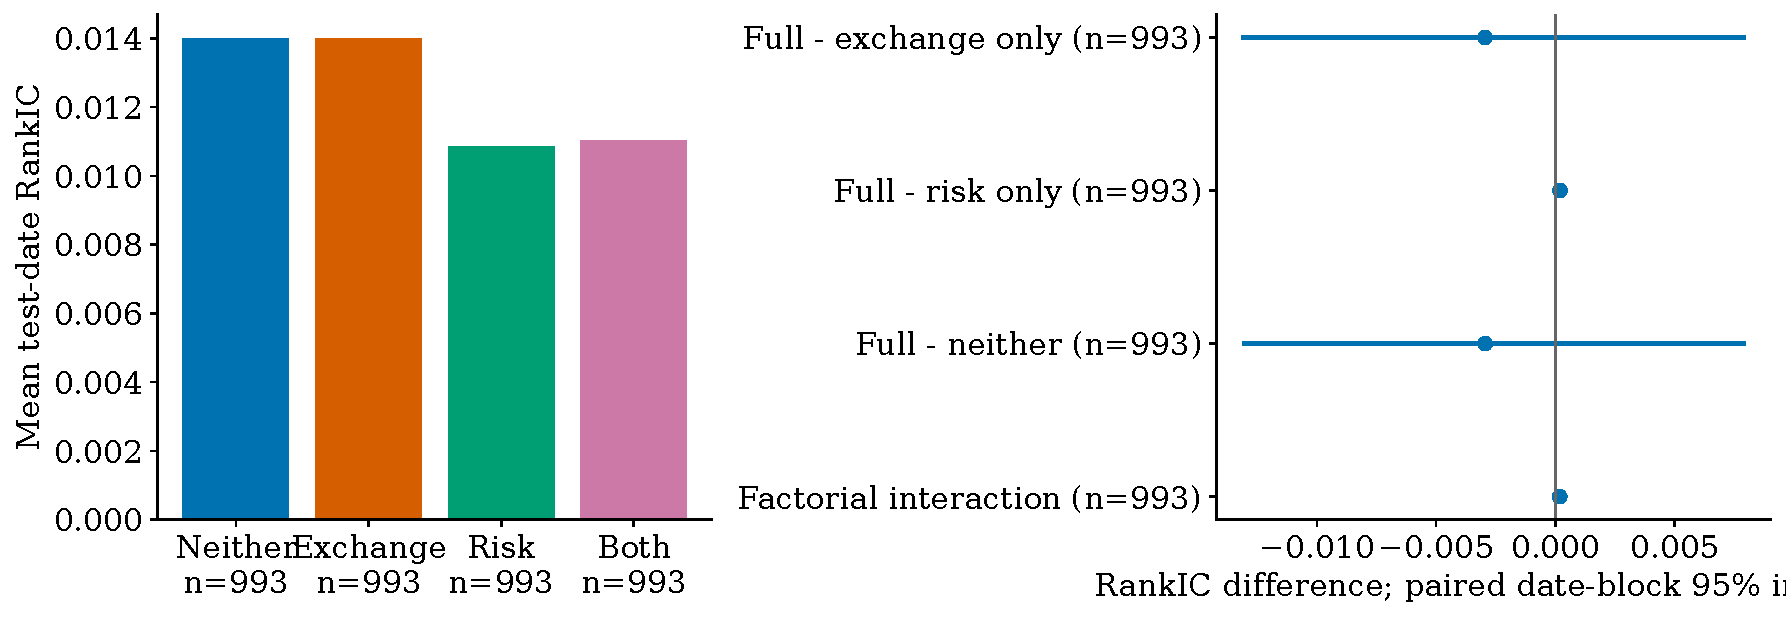
\includegraphics[width=\linewidth]{c3r_sp500_factorial.pdf}\\[-1mm]\scriptsize (a) C3R\end{minipage}\hfill
\begin{minipage}{0.32\textwidth}\centering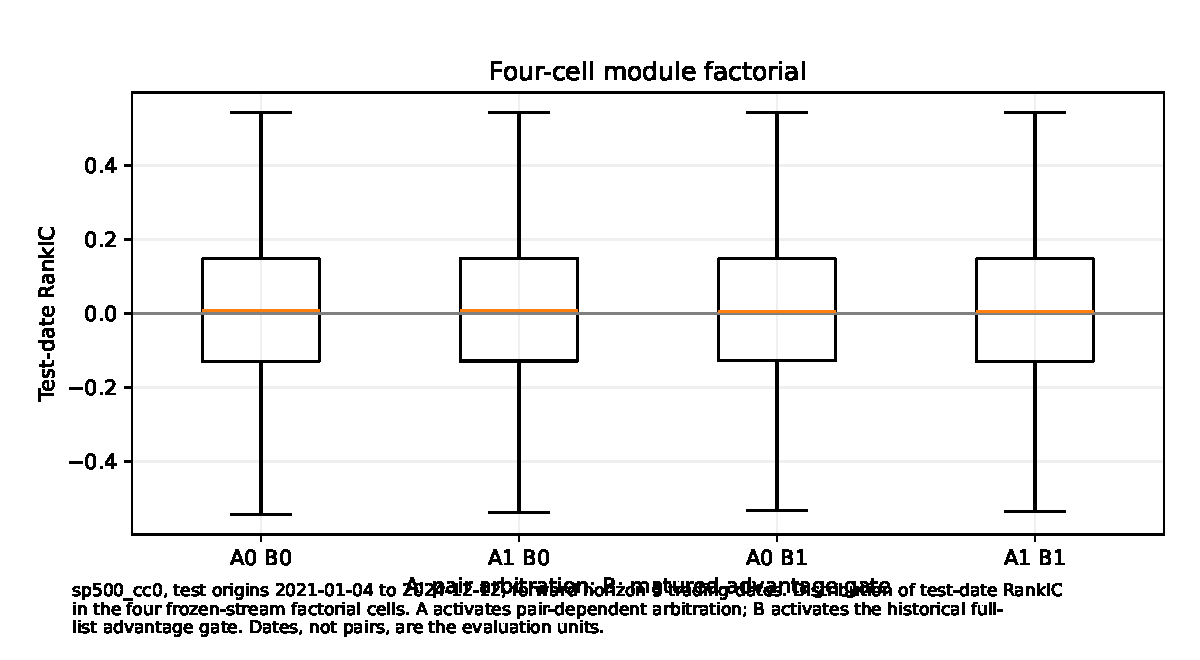
\includegraphics[width=\linewidth]{darc_sp500_factorial.pdf}\\[-1mm]\scriptsize (b) DARC\end{minipage}\hfill
\begin{minipage}{0.32\textwidth}\centering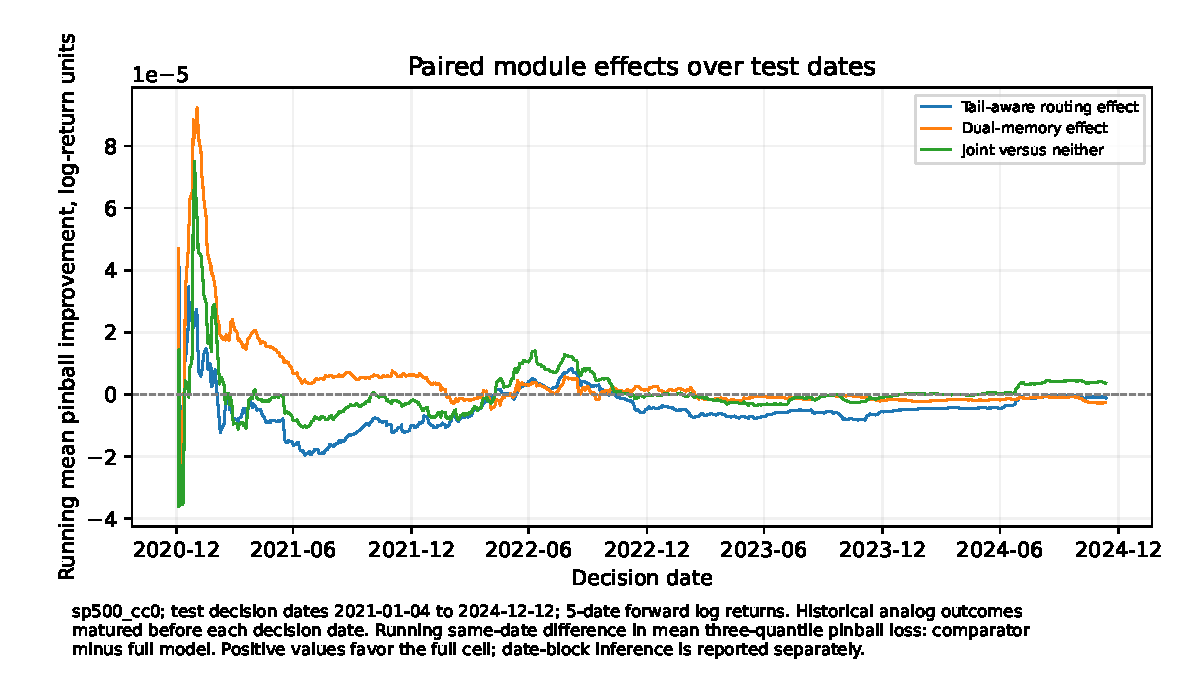
\includegraphics[width=\linewidth]{care_sp500_factorial.pdf}\\[-1mm]\scriptsize (c) CARE\end{minipage}
\caption{Factorial evidence for C3R, DARC, and CARE on SP500. The panels use their original task-specific scales. They illustrate activation and component contrasts; cross-study visual heights are not comparable.}
\label{fig:factorial1}
\end{figure}

\begin{figure}[H]
\centering
\begin{minipage}{0.48\textwidth}\centering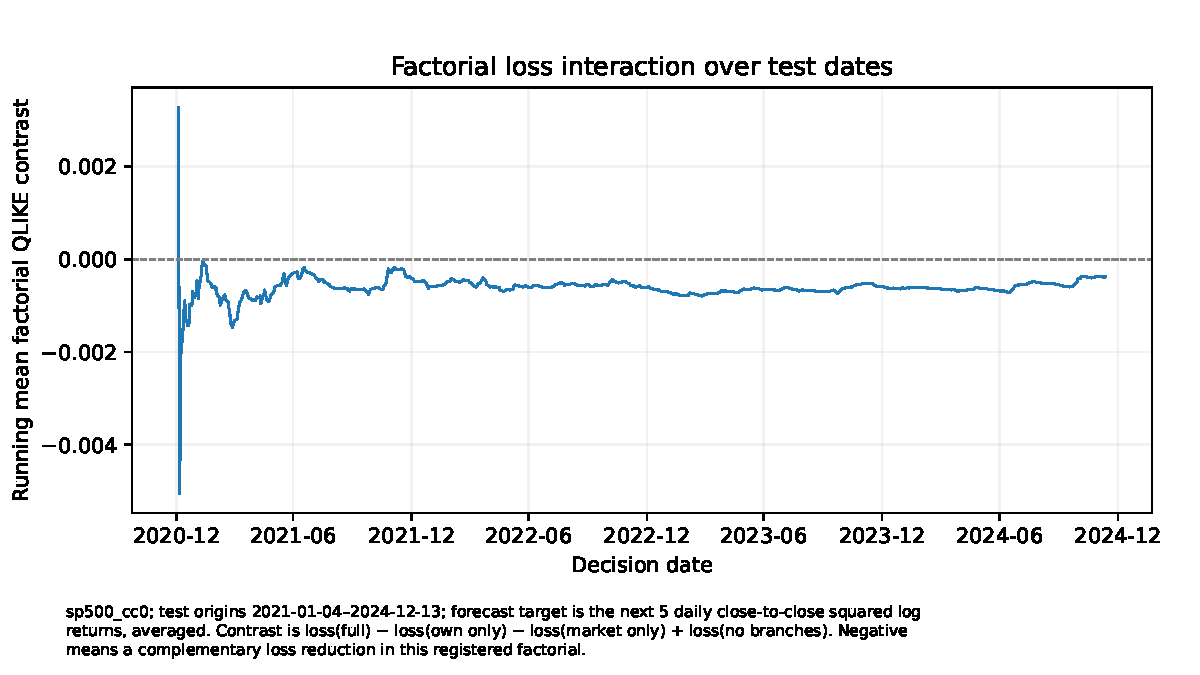
\includegraphics[width=\linewidth]{mosaic_sp500_factorial.pdf}\\[-1mm]\scriptsize (a) MOSAIC\end{minipage}\hfill
\begin{minipage}{0.48\textwidth}\centering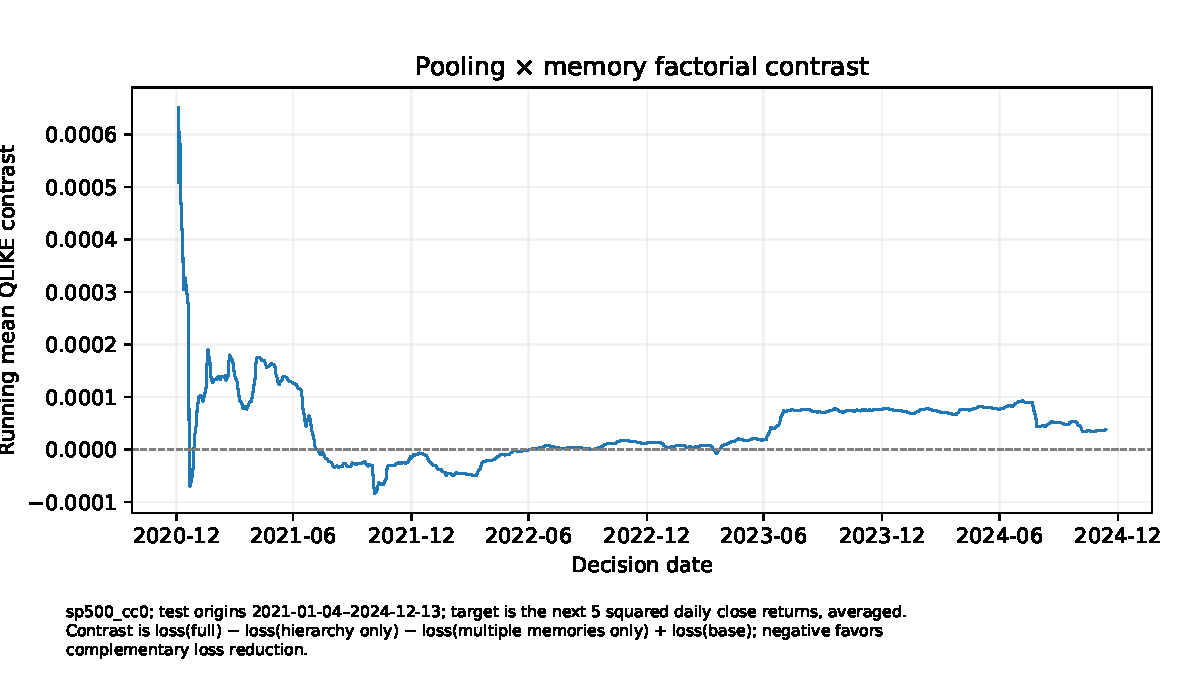
\includegraphics[width=\linewidth]{dashv_sp500_factorial.pdf}\\[-1mm]\scriptsize (b) DASH-V\end{minipage}
\caption{Factorial evidence for MOSAIC and DASH-V on SP500. Both studies target the same daily-return variance proxy, but use different models and comparator families.}
\label{fig:factorial2}
\end{figure}

\subsection{Activation was common; useful differentiation was not}

The completed archives separate operational integrity from predictive contribution. Every recorded fit completed and every proposed cell produced finite predictions, allowing the analysis to locate where an active mechanism stopped creating forecast value.

Figure~\ref{fig:mechanism-diagnostics} reports one representative test-period diagnostic for each model. Each panel tests an intermediate restriction required by the model's story; the paragraphs below connect that restriction to the matched forecasting result.

\begin{figure}[H]
\centering
\begin{minipage}{0.485\textwidth}\centering
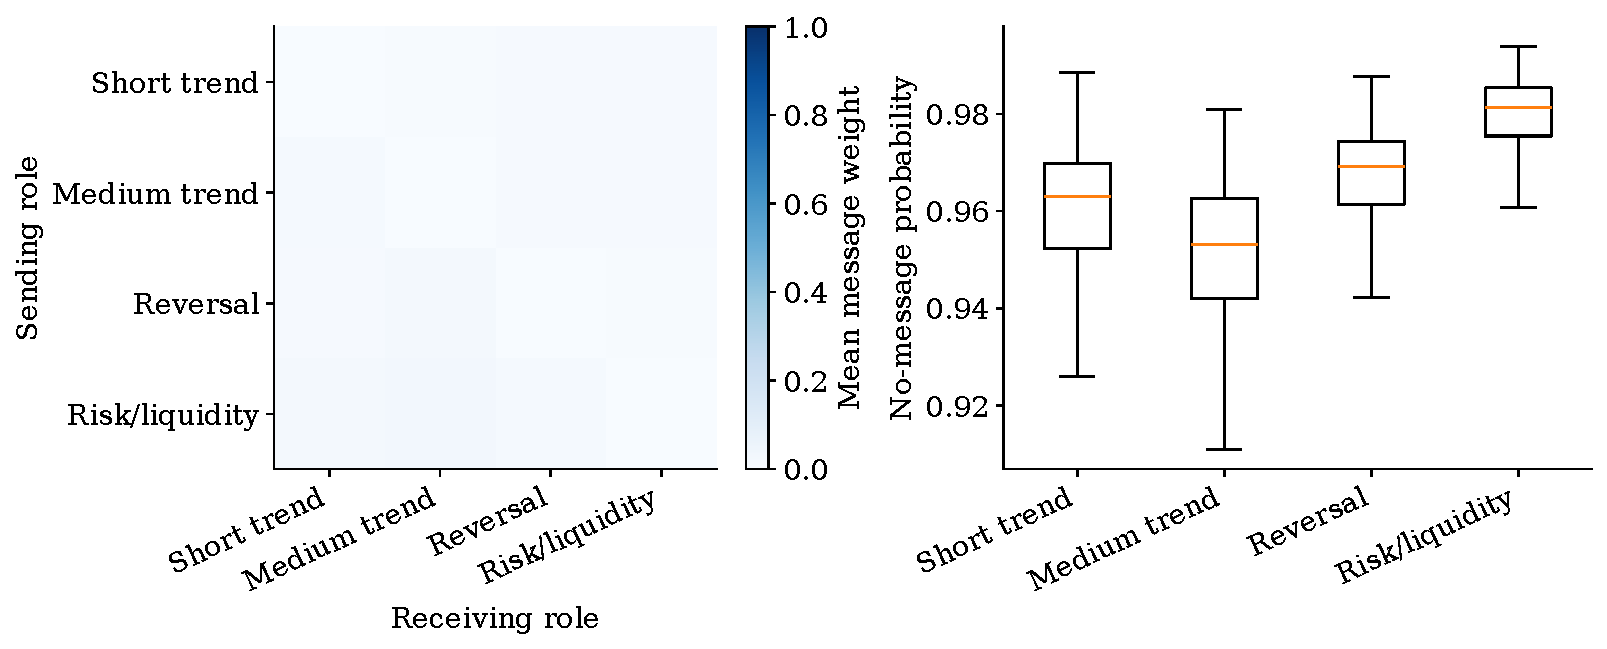
\includegraphics[width=\linewidth]{c3r_sp500_communication_abstention.pdf}\\[-1mm]\scriptsize (a) C3R
\end{minipage}\hfill
\begin{minipage}{0.485\textwidth}\centering
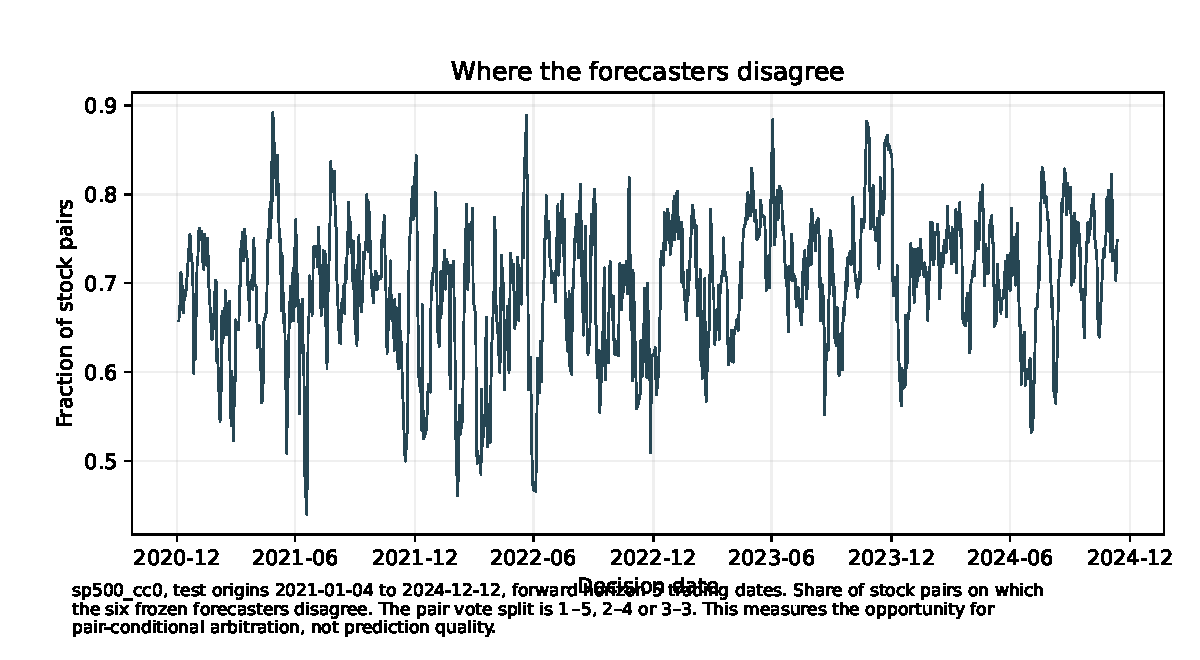
\includegraphics[width=\linewidth]{darc_sp500_disagreement.pdf}\\[-1mm]\scriptsize (b) DARC
\end{minipage}\\[2mm]
\begin{minipage}{0.485\textwidth}\centering
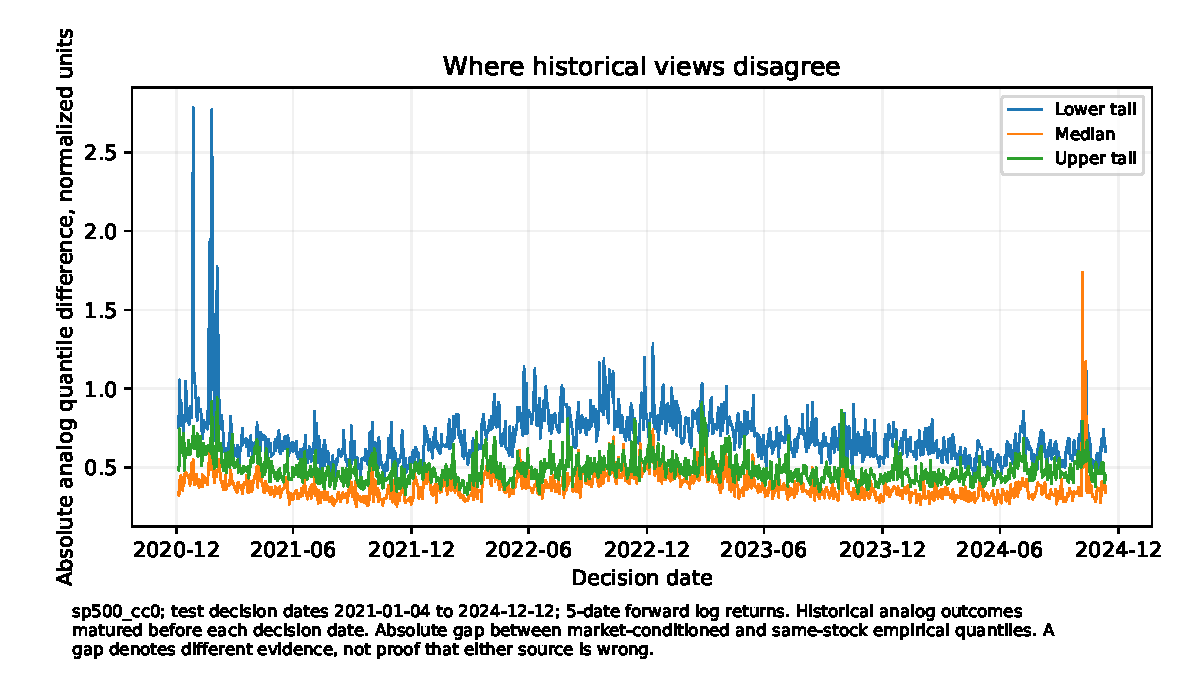
\includegraphics[width=\linewidth]{care_sp500_memory_disagreement.pdf}\\[-1mm]\scriptsize (c) CARE
\end{minipage}\hfill
\begin{minipage}{0.485\textwidth}\centering
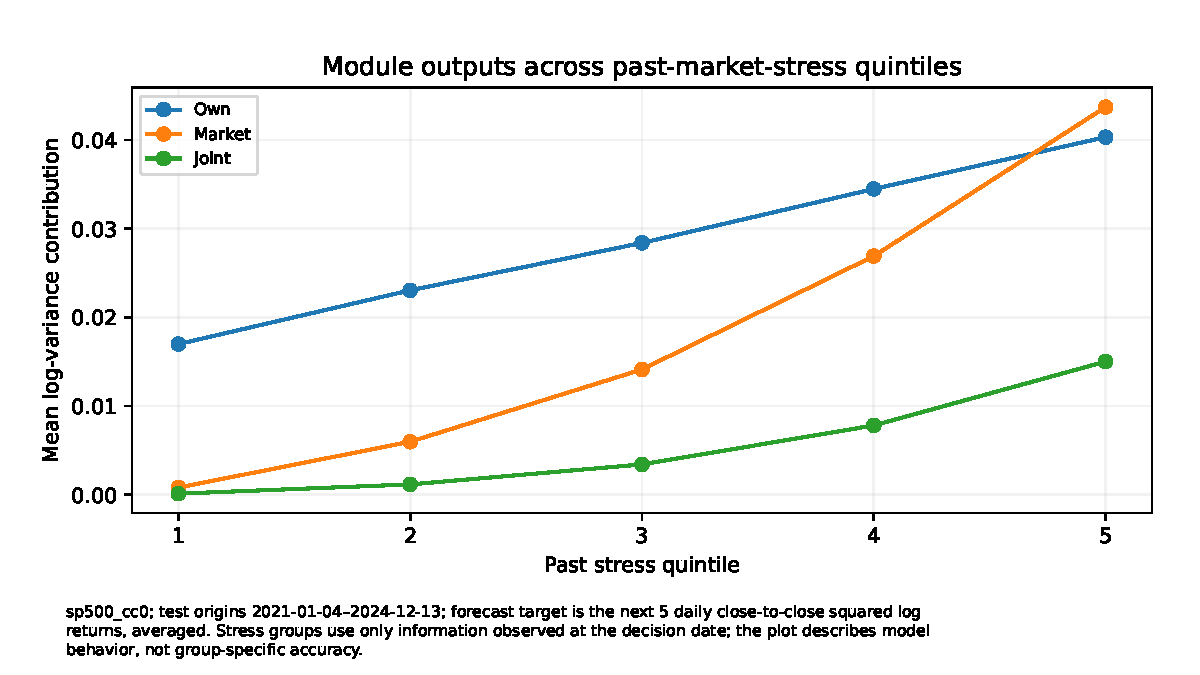
\includegraphics[width=\linewidth]{mosaic_sp500_stress.pdf}\\[-1mm]\scriptsize (d) MOSAIC
\end{minipage}\\[2mm]
\begin{minipage}{0.485\textwidth}\centering
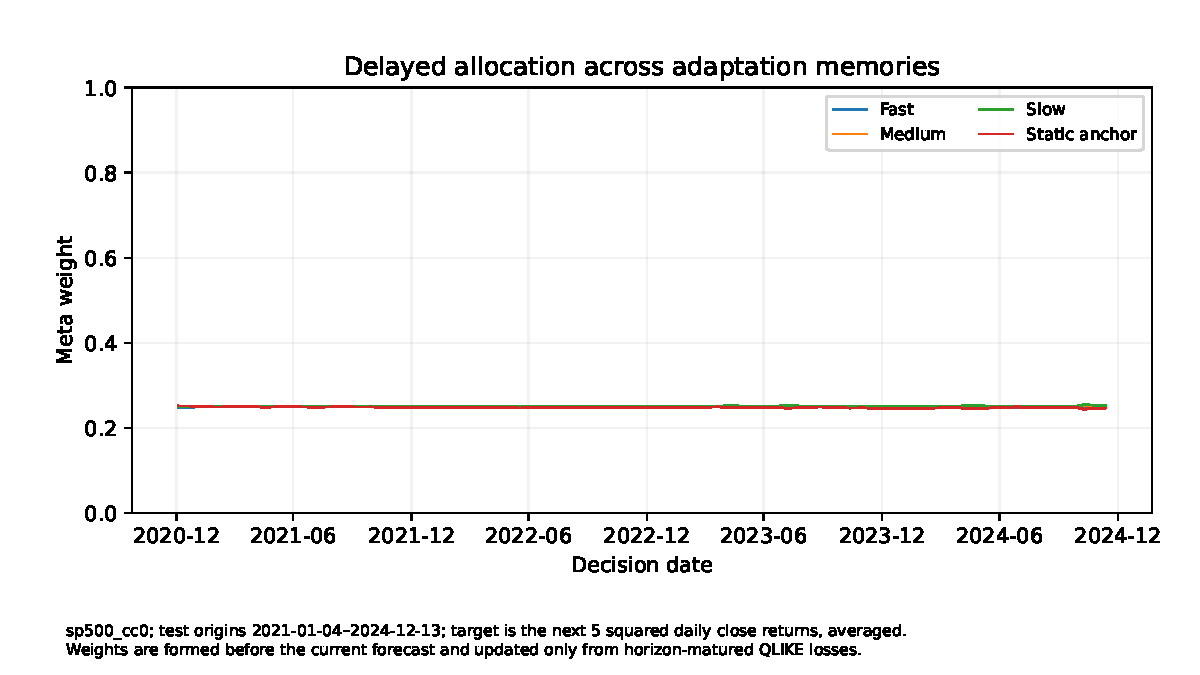
\includegraphics[width=\linewidth]{dashv_sp500_memory_weights.pdf}\\[-1mm]\scriptsize (e) DASH-V
\end{minipage}
\caption{Representative SP500 activation diagnostics: C3R communication and abstention, DARC forecast disagreement, CARE cross-memory quantile gaps, MOSAIC stress-conditioned branch responses, and DASH-V delayed memory allocation. All panels use archived test-period outputs. They diagnose whether the intended channel operated; Table~\ref{tab:main} and Figures~\ref{fig:factorial1}--\ref{fig:factorial2} determine forecast value.}
\label{fig:mechanism-diagnostics}
\end{figure}

In C3R, null-message probabilities were high and message energy was tiny. The candidate communication coalitions consequently produced nearly identical losses. A predeclared normalization floor exceeded the observed candidate-loss dispersion on every cached training date, compressing the routing target. The route weights became close to uniform. Residual exchange was intended to suppress duplicated latent information, but the same conservative design also reduced the variation that the coalition-risk router needed to learn. The mechanism therefore reached the representation stage without generating a sufficiently separated decision problem.

In decision terms, coalition-loss dispersion is the signal available to distinguish routing actions. Once that dispersion lies below the normalization scale, uniform-like weights are the expected regularized solution rather than evidence of successful conditional selection.

In DARC, the gate retained roughly half the candidate corrections by construction, but the bank of expert weights was only weakly differentiated. Pairwise correctness did not reliably translate into a better completed ranking. Pairwise arbitration can help when local preferences are stable and sufficiently transitive; here, small local advantages dissipated during rank completion. The missing fixed-half-mixture control also limited attribution: a gate that admits half the interventions should be compared with a matched rule that admits the same fraction without using the proposed signal.

Rank completion is a nonlinear aggregation step: locally favorable pair decisions can form cycles or cancel across assets. The experiment therefore evaluates the completed date-level ordering, rather than counting pairwise decisions as if they were independent successes.

CARE's two memories returned different analog sets and the routes changed across dates. The center-plus-positive-width parameterization maintained ordered quantiles, so the negative comparison cannot be attributed to quantile crossing. Instead, cross-memory differences did not reliably identify which distribution component should depart from the shared temporal forecast. The full tail-sensitive route was not consistently better than the dual-memory plain route or the best common-protocol quantile model.

For a tail selector, the relevant quantity is not disagreement alone but its alignment with the later component-specific pinball gradient. Large analog differences can be reproducible yet unhelpful when neither memory is systematically closer to the realized tail.

MOSAIC's correction branches changed the anchor and improved it slightly. The anchor--correction decomposition preserved positivity and isolated asymmetric stress, but the interaction did not show that joint stock and market stress added information beyond the two marginal branches. The anchor family itself was weaker than several controls.

This separates correction alignment from family adequacy. A branch may lower QLIKE relative to its own anchor while the remaining anchor error is still larger than the error of an equally informed external model.

DASH-V moved away from static pooling, but its memory weights stayed close to one quarter for fast, medium, slow, and static components. Partial pooling was designed to trade the responsiveness of local short memories against the stability of global histories. The near-equal allocation indicates that matured relative losses supplied too little persistent separation to justify decisive adaptation. An adaptive layer can therefore change forecasts while remaining close to fixed averaging in the dimension central to its story.

Delayed labels reduce the effective evidence in the fastest memory, while long memories average across potential regime changes. Multi-scale pooling helps only when the observed loss gaps persist long enough to be learned after maturity and remain relevant at deployment.

\section{Discussion}

\subsection{A matched reduction is often the decisive baseline}

The strongest diagnostic comparator was rarely the oldest or simplest forecast. It was the reduction that kept the same information and training opportunity while removing the proposed interaction. C3R needed a risk-only router; DARC needed a global weighted-rank reduction and a fixed-adoption control; CARE needed single-memory and dual-memory plain routes; MOSAIC needed an anchor-only family; DASH-V needed static and equal-memory pools. Such controls distinguish extra information from extra computation.

\subsection{Simple controls remain hard to beat}

Financial panels contain strong persistence, common shocks, and unstable cross-sectional relations. These properties favor simple rules that estimate few moving parts. The result is not a universal argument against neural models or ensembles. It is an argument for treating static pooling, persistence, HAR-type regressions, equal-rank combinations, and frozen single models as first-class comparators. When a complex mechanism wins only against its own weakened base, the paper should say so directly.

\subsection{A five-regime diagnostic map}

The five studies do not fail in one generic way. C3R is closest to \emph{dormancy}: conservative residual messages and a normalization floor left candidate coalition risks too similar for decisive routing. DARC is closer to \emph{non-translation}: forecasters disagreed and the gate operated, but local pair decisions did not reliably improve the final ranking. CARE illustrates \emph{redundant activity}: two memories retrieved different episodes and changed the routes, yet those distinctions did not add proper-score value beyond simpler alternatives. MOSAIC shows \emph{family weakness}: its corrections improved the chosen anchor, while stronger models outside that family retained lower QLIKE. DASH-V shows \emph{adaptive contraction}: the delayed hierarchy moved forecasts but validation-estimated shrinkage and near-equal memory allocation limited the practical departure from static pooling.

This taxonomy turns adverse evidence into a redesign map. Dormancy calls for rescaling or a more informative routing target; non-translation calls for a readout tied more directly to the final score; redundancy calls for a conditional test of when two information sources differ; family weakness calls for a stronger anchor before another correction branch is added; adaptive contraction calls for evidence that regimes change fast enough to reward adaptation. The categories distinguish failures of representation, selection, forecast family, and deployment, so they prescribe different next experiments rather than another undirected increase in model capacity.

\subsection{Implications for model governance and financial use}

The audit also has a practical governance interpretation. Institutions compare an advanced system with a maintained benchmark whose behavior and cost are known. Same-information reductions estimate what the extra mechanism buys before implementation and model-risk costs are added. Internal diagnostics can then monitor whether routing, expert weights, memory allocation, or correction magnitudes leave their calibrated range, while matured outcomes and benchmark comparisons continue to determine forecast value. Preserving adverse panels makes the resulting control more specific: dormancy calls for an activation check, redundancy for a cost justification, family weakness for a stronger base forecast, and unstable selection for a conservative fallback.

\section{Limitations}

The synthesis has five material limits. First, the studies share panels and were developed sequentially, so the study--panel cells are dependent. Second, the tasks and primary scores differ; no common effect size is available. Third, the named neural architectures are common-protocol adaptations rather than full reproductions of original-author pipelines. Fourth, SP500 uses current constituents and therefore cannot represent a survivorship-free historical index universe. Fifth, the evidence comes from daily public panels and modest training budgets. The results do not show that the mechanisms fail in every market, at every frequency, or under substantially larger training regimes.

These limits narrow the claim but do not erase the evidence. The relevant conclusion is about the completed implementations under their recorded information sets and controls. Every adverse panel is retained, and no secondary metric is used to overturn a failed primary comparison.

\section{Conclusion}

Five technically complete studies tested five different ways to make financial forecasts more adaptive. None established broad superiority across the three public panels, but the common audit identified where each value chain broke: communication became numerically dormant, routing targets were compressed, gates did not translate local correctness into final rankings, retrieval did not improve proper scores, correction branches improved a weak family, and multiple memories behaved nearly like equal allocation.

The result is a reusable method for evaluating architectural claims. A forecasting module earns a performance claim only after it beats a same-information reduction, survives date-level uncertainty estimates, clears strong controls, and retains adverse panels. Separating action diversity, loss alignment, and deployment value shows whether the next design should change the representation, selector, forecast family, or validation protocol. That evidence guides research allocation and operational use.

\section*{Data and code availability}

Study configurations, checksums, study-level result tables, code, and returned execution archives are retained in the project archive and can be shared in anonymized form subject to third-party data licenses and editorial instructions. Where redistribution is not permitted, the archive supplies acquisition instructions, source identifiers, and file hashes. Failed and adverse comparisons and the complete figure sets remain indexed. The SP500 limitation described above applies to every study that uses it.

\section*{Funding}

No external funding is declared in the anonymous submission.

\section*{Conflict of interest}

The author(s) declare no conflict of interest.

\bibliography{references}

\end{document}
